\subsection{MoM Longitudinal Acceleration}
\label{sec:eval_req_mom_long}

\subsubsection{Configuration}

\begin{figure}[H]
    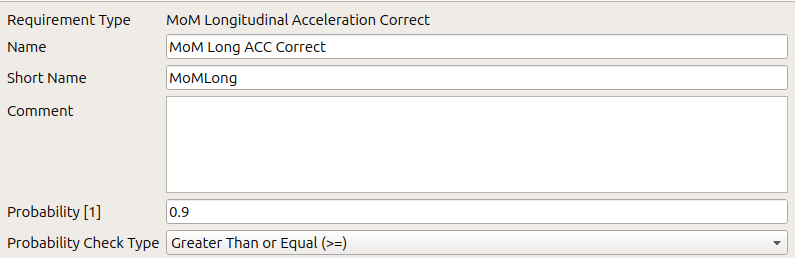
\includegraphics[width=14cm,frame]{figures/eval_req_mom_long.png}
  \caption{Evaluation MoM Longitudinal Acceleration Requirement}
\end{figure}

The 'MoM Longitudinal Acceleration’ requirement is used to calculate the probability of a target report having a difference in the track Mode-of-Movement Longitudinal Acceleration enumerated type. 

\begin{itemize}  
\item Probability [1]: Probability of correct MoM enumerated type value
\item Probability Check Type: $\geq$
\end{itemize}
\ \\

\subsubsection{Calculation}

The MoM enumerated type of the test data is compared to the two reference updates closest in time (before and after the test timestamp), if one of the reference enum values matches the target report is counted for the calculated probability PCLAcc (probability of correct MoM longitudinal acceleration). The PCLAcc must be in turn pass the check for the requirement to pass. 

\subsubsection{Result Values}

\paragraph{Sector}

\begin{center}
 \begin{table}[H]
  \begin{tabularx}{\textwidth}{ | l | X |  l | }
    \hline
    \textbf{Name} & \textbf{Description} & \textbf{Example} \\ \hline
    Sector Layer & Name of the sector layer & units\_OPS\_2024 \\ \hline
    Requirement Group & Name of the requirement group & Mandatory \\ \hline
    Requirement & Name of the requirement & MoM Long ACC Correct \\ \hline
    Num Results & Total number of results & 1969 \\ \hline
    Num Usable Results & Number of usable results & 1493 \\ \hline
    Num Unusable Results & Number of unusable results & 476 \\ \hline
    Use & To be used in results & true \\ \hline
    \#Up [1] & Number of updates & 583550 \\ \hline
    \#NoRef [1] & Number of updates w/o reference position or MoM Longitudinal Acceleration & 282 \\ \hline
    \#NoRefPos [1] & Number of updates w/o reference position & 282 \\ \hline
    \#NoRef [1] & Number of updates w/o reference MoM Longitudinal Acceleration & 0 \\ \hline
    \#PosInside [1] & Number of updates inside sector & 582973 \\ \hline
    \#PosOutside [1] & Number of updates outside sector & 295 \\ \hline
    \#Unknown [1] & Number of updates unknown MoM Longitudinal Acceleration & 0 \\ \hline
    \#Correct [1] & Number of updates with correct MoM Longitudinal Acceleration & 479871 \\ \hline
    \#False [1] & Number of updates with incorrect MoM Longitudinal Acceleration & 103102 \\ \hline
    PCLAcc [\%] & Probability of Correct MoM Longitudinal Acceleration & 82.31 \\ \hline
    Condition &  & >= 90.00 \\ \hline
    Condition Fulfilled &  & Failed \\ \hline
    \end{tabularx}
\end{table}
\end{center}

Also, a table is given for all single targets, sorted by PCLAcc.

\paragraph{Single Target}

\begin{center}
 \begin{table}[H]
  \begin{tabularx}{\textwidth}{ | l | X |  l | }
    \hline
    \textbf{Name} & \textbf{Description} & \textbf{Example} \\ \hline
    Use & To be used in results & true \\ \hline
    \#Up [1] & Number of updates & 740 \\ \hline
    \#NoRef [1] & Number of updates w/o reference position or MoM Longitudinal Acceleration & 0 \\ \hline
    \#NoRefPos [1] & Number of updates w/o reference position  & 0 \\ \hline
    \#NoRef [1] & Number of updates w/o reference MoM Longitudinal Acceleration & 0 \\ \hline
    \#PosInside [1] & Number of updates inside sector & 740 \\ \hline
    \#PosOutside [1] & Number of updates outside sector & 0 \\ \hline
    \#Unknown [1] & Number of updates unknown MoM Longitudinal Acceleration & 0 \\ \hline
    \#Correct [1] & Number of updates with correct MoM Longitudinal Acceleration & 569 \\ \hline
    \#False [1] & Number of updates with incorrect MoM Longitudinal Acceleration & 171 \\ \hline
    PCLAcc [\%] & Probability of Correct MoM Longitudinal Acceleration & 76.89 \\ \hline
    Condition &  & >= 90.00 \\ \hline
    Condition Fulfilled &  & Failed \\ \hline
\end{tabularx}
\end{table}
\end{center}


\subsection{MoM Transversal Acceleration}
\label{sec:eval_req_mom_trans}

\subsubsection{Configuration}

\begin{figure}[H]
    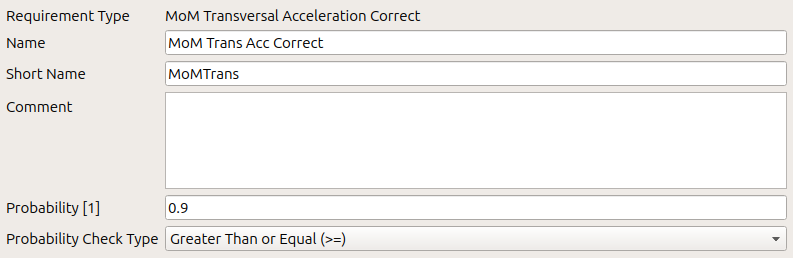
\includegraphics[width=14cm,frame]{figures/eval_req_mom_trans.png}
  \caption{Evaluation MoM Transversal Acceleration Requirement}
\end{figure}

The 'MoM Transversal Acceleration’ requirement is used to calculate the probability of a target report having a difference in the track Mode-of-Movement Transversal Acceleration enumerated type. 

\begin{itemize}  
\item Probability [1]: Probability of correct MoM enumerated type value
\item Probability Check Type: $\geq$
\end{itemize}
\ \\

\subsubsection{Calculation}

The MoM enumerated type of the test data is compared to the two reference updates closest in time (before and after the test timestamp), if one of the reference enum values matches the target report is counted for the calculated probability PCLAcc (probability of correct MoM longitudinal acceleration). The PCLAcc must be in turn pass the check for the requirement to pass. 

\subsubsection{Result Values}

\paragraph{Sector}

\begin{center}
 \begin{table}[H]
  \begin{tabularx}{\textwidth}{ | l | X |  l | }
    \hline
    \textbf{Name} & \textbf{Description} & \textbf{Example} \\ \hline
    Sector Layer & Name of the sector layer & units\_OPS\_2024 \\ \hline
    Requirement Group & Name of the requirement group & Mandatory \\ \hline
    Requirement & Name of the requirement & MoM Trans Acc Correct \\ \hline
    Num Results & Total number of results & 1969 \\ \hline
    Num Usable Results & Number of usable results & 1493 \\ \hline
    Num Unusable Results & Number of unusable results & 476 \\ \hline
    Use & To be used in results & true \\ \hline
    \#Up [1] & Number of updates & 583550 \\ \hline
    \#NoRef [1] & Number of updates w/o reference position or MoM Transversal Acceleration & 282 \\ \hline
    \#NoRefPos [1] & Number of updates w/o reference position & 282 \\ \hline
    \#NoRef [1] & Number of updates w/o reference MoM Transversal Acceleration & 0 \\ \hline
    \#PosInside [1] & Number of updates inside sector & 582973 \\ \hline
    \#PosOutside [1] & Number of updates outside sector & 295 \\ \hline
    \#Unknown [1] & Number of updates unknown MoM Transversal Acceleration & 0 \\ \hline
    \#Correct [1] & Number of updates with correct MoM Transversal Acceleration & 573156 \\ \hline
    \#False [1] & Number of updates with incorrect MoM Transversal Acceleration & 9817 \\ \hline
    PCTAcc [\%] & Probability of Correct MoM Transversal Acceleration & 98.32 \\ \hline
    Condition &  & >= 90.00 \\ \hline
    Condition Fulfilled &  & Passed \\ \hline
    \end{tabularx}
\end{table}
\end{center}

Also, a table is given for all single targets, sorted by PCTAcc.

\paragraph{Single Target}

\begin{center}
 \begin{table}[H]
  \begin{tabularx}{\textwidth}{ | l | X |  l | }
    \hline
    \textbf{Name} & \textbf{Description} & \textbf{Example} \\ \hline
    Use & To be used in results & true \\ \hline
    \#Up [1] & Number of updates & 740 \\ \hline
    \#NoRef [1] & Number of updates w/o reference position or MoM Transversal Acceleration & 0 \\ \hline
    \#NoRefPos [1] & Number of updates w/o reference position  & 0 \\ \hline
    \#NoRef [1] & Number of updates w/o reference MoM Transversal Acceleration & 0 \\ \hline
    \#PosInside [1] & Number of updates inside sector & 740 \\ \hline
    \#PosOutside [1] & Number of updates outside sector & 0 \\ \hline
    \#Unknown [1] & Number of updates unknown MoM Transversal Acceleration & 0 \\ \hline
    \#Correct [1] & Number of updates with correct MoM Transversal Acceleration & 740 \\ \hline
    \#False [1] & Number of updates with incorrect MoM Transversal Acceleration & 0 \\ \hline
    PCTAcc [\%] & Probability of Correct MoM Transversal Acceleration & 100.00 \\ \hline
    Condition &  & >= 90.00 \\ \hline
    Condition Fulfilled &  & Passed \\ \hline
\end{tabularx}
\end{table}
\end{center}


\subsection{MoM Vertical Rate}
\label{sec:eval_req_mom_vert}

\subsubsection{Configuration}

\begin{figure}[H]
    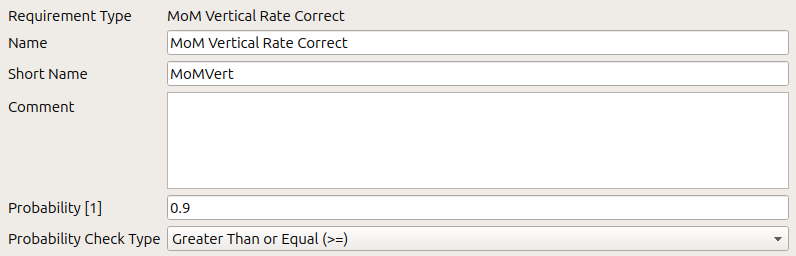
\includegraphics[width=14cm,frame]{figures/eval_req_mom_vert.png}
  \caption{Evaluation MoM Vertical Rate Requirement}
\end{figure}

The 'MoM Vertical Rate’ requirement is used to calculate the probability of a target report having a difference in the track Mode-of-Movement Vertical Rate enumerated type. 

\begin{itemize}  
\item Probability [1]: Probability of correct MoM enumerated type value
\item Probability Check Type: $\geq$
\end{itemize}
\ \\


\subsubsection{Calculation}

The MoM enumerated type of the test data is compared to the two reference updates closest in time (before and after the test timestamp), if one of the reference enum values matches the target report is counted for the calculated probability PCVRt (probability of correct MoM vertical rate). The PCVRt must in turn pass the check for the requirement to pass. 

\subsubsection{Result Values}

\paragraph{Sector}

\begin{center}
 \begin{table}[H]
  \begin{tabularx}{\textwidth}{ | l | X |  l | }
    \hline
    \textbf{Name} & \textbf{Description} & \textbf{Example} \\ \hline
    Sector Layer & Name of the sector layer & units\_OPS\_2024 \\ \hline
    Requirement Group & Name of the requirement group & Mandatory \\ \hline
    Requirement & Name of the requirement & MoM Vertical Rate Correct \\ \hline
    Num Results & Total number of results & 1969 \\ \hline
    Num Usable Results & Number of usable results & 1493 \\ \hline
    Num Unusable Results & Number of unusable results & 476 \\ \hline
    Use & To be used in results & true \\ \hline
    \#Up [1] & Number of updates & 583550 \\ \hline
    \#NoRef [1] & Number of updates w/o reference position or MoM Vertical Rate & 282 \\ \hline
    \#NoRefPos [1] & Number of updates w/o reference position & 282 \\ \hline
    \#NoRef [1] & Number of updates w/o reference MoM Vertical Rate & 0 \\ \hline
    \#PosInside [1] & Number of updates inside sector & 582973 \\ \hline
    \#PosOutside [1] & Number of updates outside sector & 295 \\ \hline
    \#Unknown [1] & Number of updates unknown MoM Vertical Rate & 0 \\ \hline
    \#Correct [1] & Number of updates with correct MoM Vertical Rate & 530018 \\ \hline
    \#False [1] & Number of updates with incorrect MoM Vertical Rate & 52955 \\ \hline
    PCVRt [\%] & Probability of Correct MoM Vertical Rate & 90.92 \\ \hline
    Condition &  & >= 90.00 \\ \hline
    Condition Fulfilled &  & Passed \\ \hline
\end{tabularx}
\end{table}
\end{center}

Also, a table is given for all single targets, sorted by PCVRt.

\paragraph{Single Target}

\begin{center}
 \begin{table}[H]
  \begin{tabularx}{\textwidth}{ | l | X |  l | }
    \hline
    \textbf{Name} & \textbf{Description} & \textbf{Example} \\ \hline
    Use & To be used in results & true \\ \hline
    \#Up [1] & Number of updates & 740 \\ \hline
    \#NoRef [1] & Number of updates w/o reference position or MoM Vertical Rate & 0 \\ \hline
    \#NoRefPos [1] & Number of updates w/o reference position  & 0 \\ \hline
    \#NoRef [1] & Number of updates w/o reference MoM Vertical Rate & 0 \\ \hline
    \#PosInside [1] & Number of updates inside sector & 740 \\ \hline
    \#PosOutside [1] & Number of updates outside sector & 0 \\ \hline
    \#Unknown [1] & Number of updates unknown MoM Vertical Rate & 0 \\ \hline
    \#Correct [1] & Number of updates with correct MoM Vertical Rate & 669 \\ \hline
    \#False [1] & Number of updates with incorrect MoM Vertical Rate & 71 \\ \hline
    PCVRt [\%] & Probability of Correct MoM Vertical Rate & 90.41 \\ \hline
    Condition &  & >= 90.00 \\ \hline
    Condition Fulfilled &  & Passed \\ \hline
\end{tabularx}
\end{table}
\end{center}
